\chapter{语言模型与文本预测}\label{语言模型与文本预测}

\section{分词器 Tokenizer 模型看到的是什么}\label{分词器 Tokenizer 模型看到的是什么}

我们决定先观察小助的输入。屏幕上是一段中文题目，进入模型的却是一串整数。这些整数不是天然对应每个汉字，也不一定对应一个完整单词；它们是分词器（tokenizer）按词表规则把文本切分后得到的词元标识符（token identifier，token ID）；后文沿用 token 和 token ID。

我们用一个极小例子理解子词分词。若词表保存完整英文单词，遇到从未见过的复合词就很难处理；若只保存字符，序列又会变长。字节对编码（Byte Pair Encoding，BPE）一类方法从小单元出发，逐步合并常见相邻片段，在词表大小与序列长度之间折中。实际 tokenizer 还有字节回退、预处理和特殊标记等差异。

一个经典的例子：我们输入 strawberry，想让小助数出字母 r 的个数。人眼可以直接扫描字符；模型可能看到几个子词片段（比如 staw 和 berry 两个 token，而不是 s t r a w\ldots 这样把每个字母都切分开），模型就需要把片段重新关联到字符，再执行计数，比如模型可能知道berry 这个 token 和字母 r 是有关系的，然后就会思考berry这个 token 由哪几个字母token 组成，模型能够做到这一点，可能是因为预训练数据中有一些关于单词拼写的语料，或者后训练中有专项训练。分词让任务的表示过程更绕，许多模型都会数错，但不能断言模型一定数错：模型可以通过训练、内部计算或外部工具完成任务。这个例子说明的是输入文本的粒度与模型理解的任务粒度是不同的。

对话还有一层常被忽略的编码。我们在界面里看见 系统（system）、用户（user）、助手（assistant）三种角色，模型实际接收的通常是由对话模板（chat template）拼成的序列，其中含有角色边界、轮次结束和生成起点等标记。角色名称可能是普通文本与特殊 token 的组合，不是所有模板都把每个角色名设为一个特殊 token。建议在AI的帮助下看一些实际案例，理解模型如何切分或组合文本为token。

当我们问问题的时候，大模型看到的内容及其完整回答里面有许多标记，自然语言夹杂在这些标记中间，这些标记是为了方便机器区分不同的文本对话。我们问：``洗车店在 50 米外，我要洗车，是开车去还是步行过去''，许多模型会给出错误的回答，比如走过去，实际上洗车就必须开车去。下面是一个模型所看到的完整序列：

我们拆解一下具体过程：

\begin{tcolorbox}[colback=gray!10, colframe=customgreen, title=对话原始文本, arc=4mm]
\textless\textbar im\_start\textbar\textgreater\allowbreak{} user\textbackslash n\allowbreak{}洗车店在 50 米外，我要洗车，是开车去还是步行过去\textless\textbar im\_end\textbar\textgreater\allowbreak{}\textbackslash n\allowbreak{}\textless\textbar im\_start\textbar\textgreater\allowbreak{} assistant\textbackslash n\allowbreak{}\textless think\textgreater\allowbreak{} 用户问的是：洗车店在50米外，要洗车，是开车去还是步行过去。\textbackslash n\allowbreak{}\textbackslash n\allowbreak{}这是一个简单的生活常识/决策问题。50米非常近，大概就是步行几十秒的距离。开车反而可能更麻烦（找停车位、倒车入库等），而且50米开过去可能一个路口都没到就到了。\textbackslash n\allowbreak{}\textbackslash n\allowbreak{}我应该给出简短、明确的建议：步行过去。理由：50米很近，步行约一分钟，开车反而费事（找车位、倒车等）。\textless/think\textgreater\allowbreak{}50米太近了，**步行过去**最省事。\textbackslash n\allowbreak{}\textbackslash n\allowbreak{}- 步行也就**几十秒到一分钟**，一脚油门一踩就过了，根本不值得专门发动车子。\textbackslash n\allowbreak{}- 开车过去还得找停车位、倒车入库，搞不好比走路还费劲。\textbackslash n\allowbreak{}- 还省了点油耗和停车费。\textbackslash n\allowbreak{}\textbackslash n\allowbreak{}所以锁好车，走过去就行，到了直接把钥匙交给店员。\textless\textbar im\_end\textbar\textgreater\allowbreak{}{}
\end{tcolorbox}

首先我们发送了一个问题，那么此时一定是对话的开始，所以自动在开头以 ``\textless\textbar im\_start\textbar\textgreater\allowbreak{} user\textbackslash n\allowbreak{}''开始，表示用户问题开始，然后拼上我们的问题，在问题结束以后自动拼上``\textless\textbar im\_end\textbar\textgreater\allowbreak{}\textbackslash n\allowbreak{}''，表示用户问题结束，接下来需要加上标记让模型知道轮到它生成，类似前面的标记，拼上``\textless\textbar im\_start\textbar\textgreater\allowbreak{} assistant\textbackslash n\allowbreak{}''，并且我们要求模型必须先思考再回答，所以加上``\textless think\textgreater\allowbreak{}''，那么模型在自己生成之前，看到的内容就是前面这些，接下来模型就自己生成一段思考内容，模型自己决定在哪里结束，在适当的位置自己拼上``\textless/think\textgreater\allowbreak{}''结束思考，接下来就是面向用户的总结回答，回答结束，模型自己拼上``\textless\textbar im\_end\textbar\textgreater\allowbreak{}''，这就是一个完整的生成过程。

图\ref{fig:对话案例}是一个比较清晰的图例，去掉标记符拆分了上面的原始文本。

\begin{figure}[t]
    \centering
    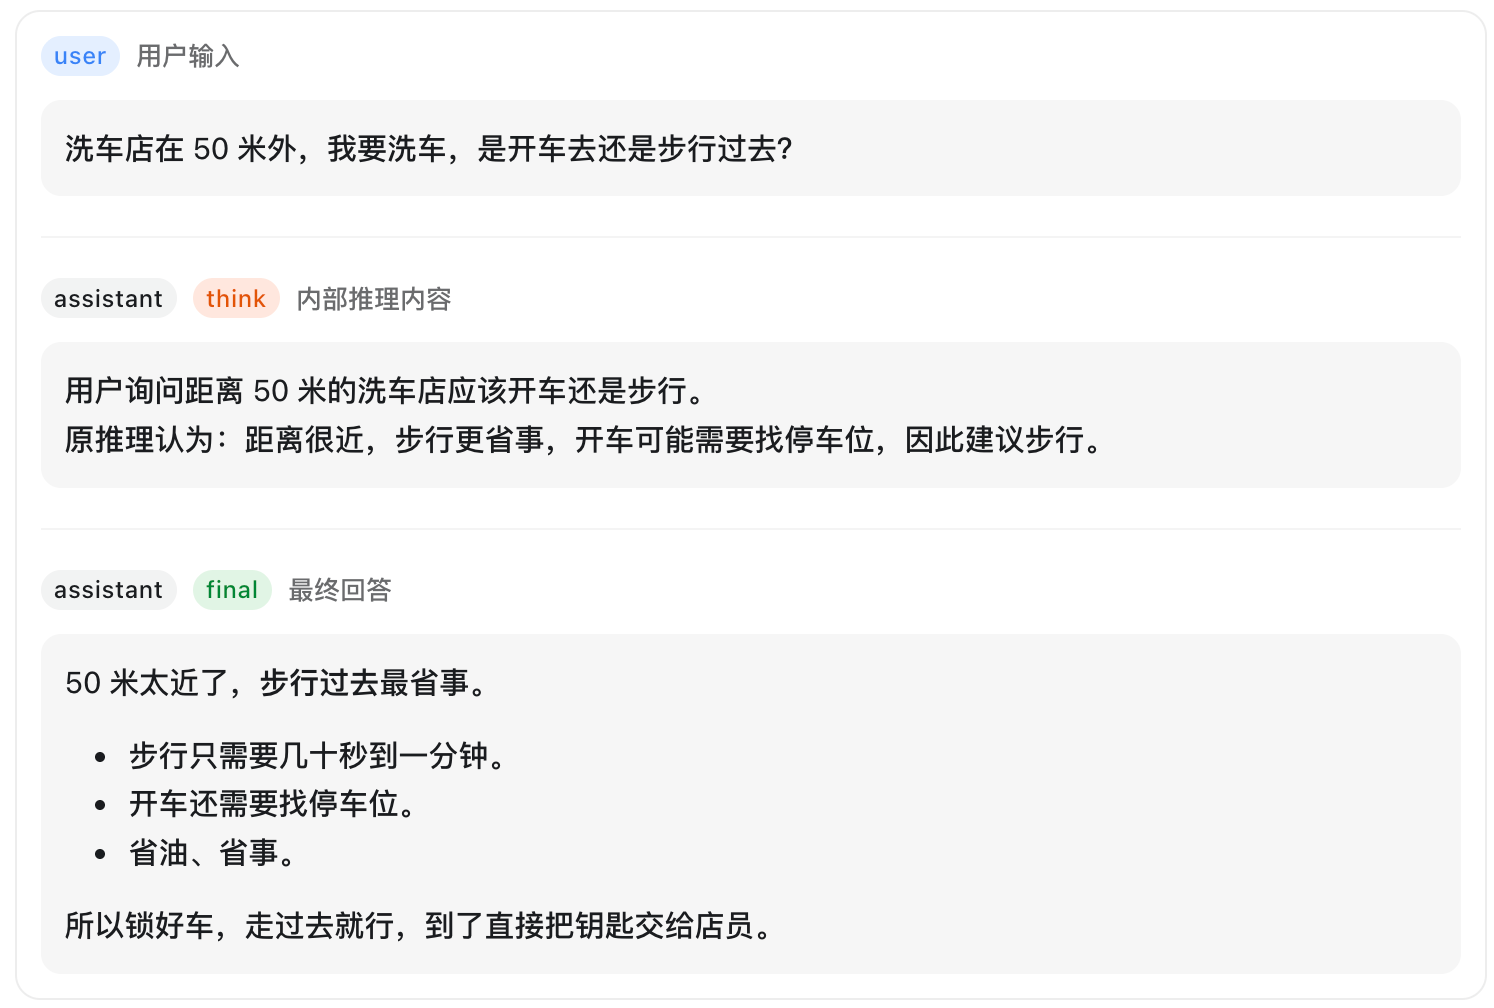
\includegraphics[width=\linewidth]{assets/media/image1.png}
    \caption{对话案例}
    \label{fig:对话案例}
\end{figure}

为什么这些标记有效，以及为什么大模型认识这些标记？模型在预训练的时候是不会见到这些标记的，但是在后训练的时候会接受大量带有这些标记的数据训练，训练之后，模型的行为分布就会变成这样，比如，不管上下文是什么，在 \textless think\textgreater\allowbreak{}{} 之后一定是思考的内容，思考完毕一定要生成一个 \textless/think\textgreater\allowbreak{}\textbackslash n\allowbreak{}\textbackslash n\allowbreak{}，然后才是给用户的回答，所以当我们要求模型进行思考时，就在模型开始推理之前拼上\textless think\textgreater\allowbreak{}，如果我们问的是一个很简单的问题，不希望模型思考，只是要模型快速回答，那么就在开始推理之前拼上\textless think\textgreater\allowbreak{}\textless/think\textgreater\allowbreak{}\textbackslash n\allowbreak{}\textbackslash n\allowbreak{}，模型就知道现在不需要思考，直接给出最终回答。我们与大模型对话的时候有一个思考开关，这个开关控制的就是这个 think 标签如何拼接在模型回答的开头。但是这个行为也是训练的概率分布，既然是概率分布就会有小概率事件，许多模型可能在 1\% 的案例中缺少 \textless/think\textgreater\allowbreak{}{} 标签或者出现其他格式错误，可能进一步造成前端显示错误。

假如训练时回答前有起始标记，推理时却漏掉起始标记，小助可能把用户内容（问题）继续写下去。假如停止标记 \textless\textbar im\_end\textbar\textgreater\allowbreak{}{} 配置错了，它可能回答完以后继续模拟用户提问，因为他不知道回答结束了，会继续写下去（因为预训练的时候问答语料可能就是这样的，在答案后面跟着下一个问题）。还有思考标记 \textless think\textgreater\allowbreak{} 也可能出问题 ，在真实工程中，有些模型的 \textless think\textgreater\allowbreak{}{} 后面一般还必须跟着两个回车（\textbackslash n\allowbreak{}\textbackslash n\allowbreak{}），如果我们的模板错了，没有这两个回车，模型的表现会打折扣，原本在一个榜单上可以做到 90分，但是因为模板错误，少了两个回车，可能就只有 85分（这种分数不一致的情况称为精度错误，其原因可能是模板错，可能是模型配置错，甚至可能和推理框架的bug有关）\textbf{。}一般来说，think 和工具等标记可能由模型自己生成，其他的标记可以由脚本自动生成，比如在模型的权重目录中有一个 chat\_template.jinja 文件来自动处理标记，这个功能也可能集成到其他的配置文件中，建议读者在huggingface或者modelscope网站中找到一些常用的开源模型，看看这些模型的文件构成。

序列长度还决定成本。同一份资料在不同 tokenizer 下可能占用不同数量的 token，因为分词规则不同；长序列会影响训练显存、截断位置、推理延迟和可用上下文。因此，``字符数''与``token数''不能互换，模型的序列长度计数是基于token的。

我们还要区分``切分有错''和``某个 token 难以生成''。MiniMax 在 2026 年公布的``马嘉祺''案例中，人们发现 Minimax M3 模型知道``马嘉祺''是谁，但是无法输出``马嘉祺''三个字。他们的研究案例提醒我们：一个词生成不出来，不足以证明 tokenizer 损坏。MiniMax 的研究者对这个问题进行了非常有参考价值的探索研究并且写成\href{https://www.minimax.cn/blog/sparse-token-forgetting-investigation}{博客}\footnote{https://www.minimax.cn/blog/sparse-token-forgetting-investigation}。

\textbf{实践} 在 OpenAI 的\href{https://platform.openai.com/tokenizer?utm_source=chatgpt.com}{分词器网站}\footnote{https://platform.openai.com/tokenizer?utm\_source=chatgpt.com}里面尝试各种文本，看看大模型是如何分词的。

\textbf{本节相关资料}
\begin{enumerate}
    \item Touvron 等，2023，\href{https://arxiv.org/abs/2307.09288}{Llama 2 Open Foundation and Fine-Tuned Chat Models} 。阅读重点：对话训练与模型使用约定如何共同影响行为。
    \item \textbf{（建议阅读）MiniMax Research，2026，\href{https://www.minimax.cn/blog/sparse-token-forgetting-investigation}{为什么 MiniMax 大模型不认识``马嘉祺'' 稀疏 Token 遗忘排查记录研究博客} 。阅读重点：如何先排除分词不一致，再检查后训练变化；与第 4.3 节对照阅读，搞清楚这个问题还需要对大模型结构有了解，比如LM head。}
\end{enumerate}

\section{下一个词元预测 NTP 从损失到信息压缩}\label{下一个词元预测 NTP 从损失到信息压缩}

本节内容对初学者来说可能比较抽象，观看 1Blue3Brown 的 \href{https://www.bilibili.com/video/BV1yVNU6xERx}{{信息压缩}}\footnote{https://www.bilibili.com/video/BV1yVNU6xERx} 视频解说可以替代本节学习。最主要的是理解这样一个观点：大模型训练可以视为信息压缩。

现在我们把小助暂时简化成一个函数：输入此前的 token，输出词表上所有候选 token 的概率。对``法国的首都是''这个前缀，它可能给``巴黎''相关的首个 token 较高概率，也给其他延续保留概率。生成时，我们从这些概率中选一个 token，接回前缀，再重复同样的过程。

这就是下一个词元预测（Next Token Prediction，NTP）。给定此前的 token，模型对下一个位置给出一个条件概率分布：
\[p_{\theta}\left( x_{t} \mid x_{< t} \right) = p_{\theta}\left( x_{t} \mid x_{1},\ldots,x_{t - 1} \right)\]

这里 θ 表示模型参数，t 表示位置，x 的下标表示序列中的 token，x 的下标小于 t 表示此前的完整前缀。对词表中所有可能的下一个 token，这些概率加起来为 1。我们不是先生成一句完整答案再给它评分，而是一步步预测。

若整段文本有 T 个 token，把这些条件概率相乘就得到序列概率。按照概率链式法则，自回归分解写为：
\[p_{\theta}\left( x_{1:T} \right) = \prod_{t = 1}^{T}p_{\theta}\left( x_{t} \mid x_{< t} \right)\]

上式中，x 的下标 1 到 T 表示整段序列，T 是序列长度，乘积号表示把各位置的条件概率相乘。每个位置都贡献一个预测任务，因此一段普通文本就能产生大量监督信号，不必另外给每个句子标上``语法课''或``事实课''。

怎样惩罚预测错误？我们取真实下一个 token 的概率，再取负对数。给正确 token 的概率越低，损失越大。若概率从 0.1 提高到 0.5，单个位置的负对数损失会从约 2.30 降到约 0.69。训练把大量位置的损失加总或平均，再用梯度更新参数。 把长度为 T 的序列在各位置的负对数概率取平均，NTP 损失写为：
\[L_{NTP} = - \frac{1}{T}\sum_{t = 1}^{T}\log p_{\theta}\left( x_{t} \mid x_{< t} \right)\]

这里 log 使用自然对数，损失的单位为 nat（奈特，自然对数的信息单位）；负号使低概率对应较大损失，前面的 1 除以 T 用来平均各位置。

为什么这个简单目标会与知识和推理有关？如果文本里出现``把 21 平均分成 3 份，每份是''，准确预测后续往往依赖算术关系；如果出现人物代词，预测可能依赖前文指代。模型可以利用词频捷径，也可能形成更可迁移的内部表示。目标并不逐条规定它必须怎样表示世界，我们要用新任务检验它究竟学到了什么。

在分布层面，交叉熵可以拆成真实数据分布的熵与一个\textbf{库尔贝克与莱布勒散度（Kullback--Leibler Divergence，KL 散度）}\footnote{KL散度是现代大模型技术中的高频概念，建议自行补充学习}。真实分布不随模型参数改变，因此最小化理想的总体交叉熵，等价于最小化数据分布到模型分布的正向 KL。有限训练集上的经验损失只是这个总体目标的估计，不能保证覆盖未见过的输入。 设 p 是真实数据分布、q 是模型分布，交叉熵与 KL 的关系具体写为：
\[H(p,q) = H(p) + D_{KL}\left( p\| q \right)\]

\(H(p,q)\) 是交叉熵，\(H(p)\) 是数据自身的熵，D 的下标 KL 表示从 p 到 q 的分布差异。p 固定时，H(p) 不随参数变化，因此优化交叉熵与优化这一 KL 项具有相同的方向。

我们已经知道，给真实 token 更高概率会降低损失。可是，为什么有人又把这说成``更会压缩''？先不急着看区间表，我们让小助承担一个具体任务：把课程文本存进文件，再从文件中逐字还原。这里讨论的是无损压缩（lossless compression），目标是在不丢失原序列的前提下减少比特数；写摘要、删掉重复句、只保留大意，都没有满足这个目标。

\textbf{先明确我们究竟在省什么} 假设消息只含 A 和 B，两者各用一个二进制位表示，100 个符号就要 100 bit。真实文本通常先由字符编码表示成字节，基线并非``一字一 bit''；我们先用二符号信源，是为了把统计结构与文本编码的细节分开。压缩器最终存下的是比特流，不是一段更短但意思差不多的自然语言。

编码器看到了原消息，解码器没有看到。两端要约定符号顺序、概率模型和消息如何结束，解码器才能从比特流唯一恢复原消息。若必须把新词表、概率表或模型权重一并发送，这些也属于总成本；只报``正文编码用了多少位''会夸大节省量。图 \ref{fig:无损压缩} 先把这份通信约定画出来：

\begin{figure}[t]
    \centering
    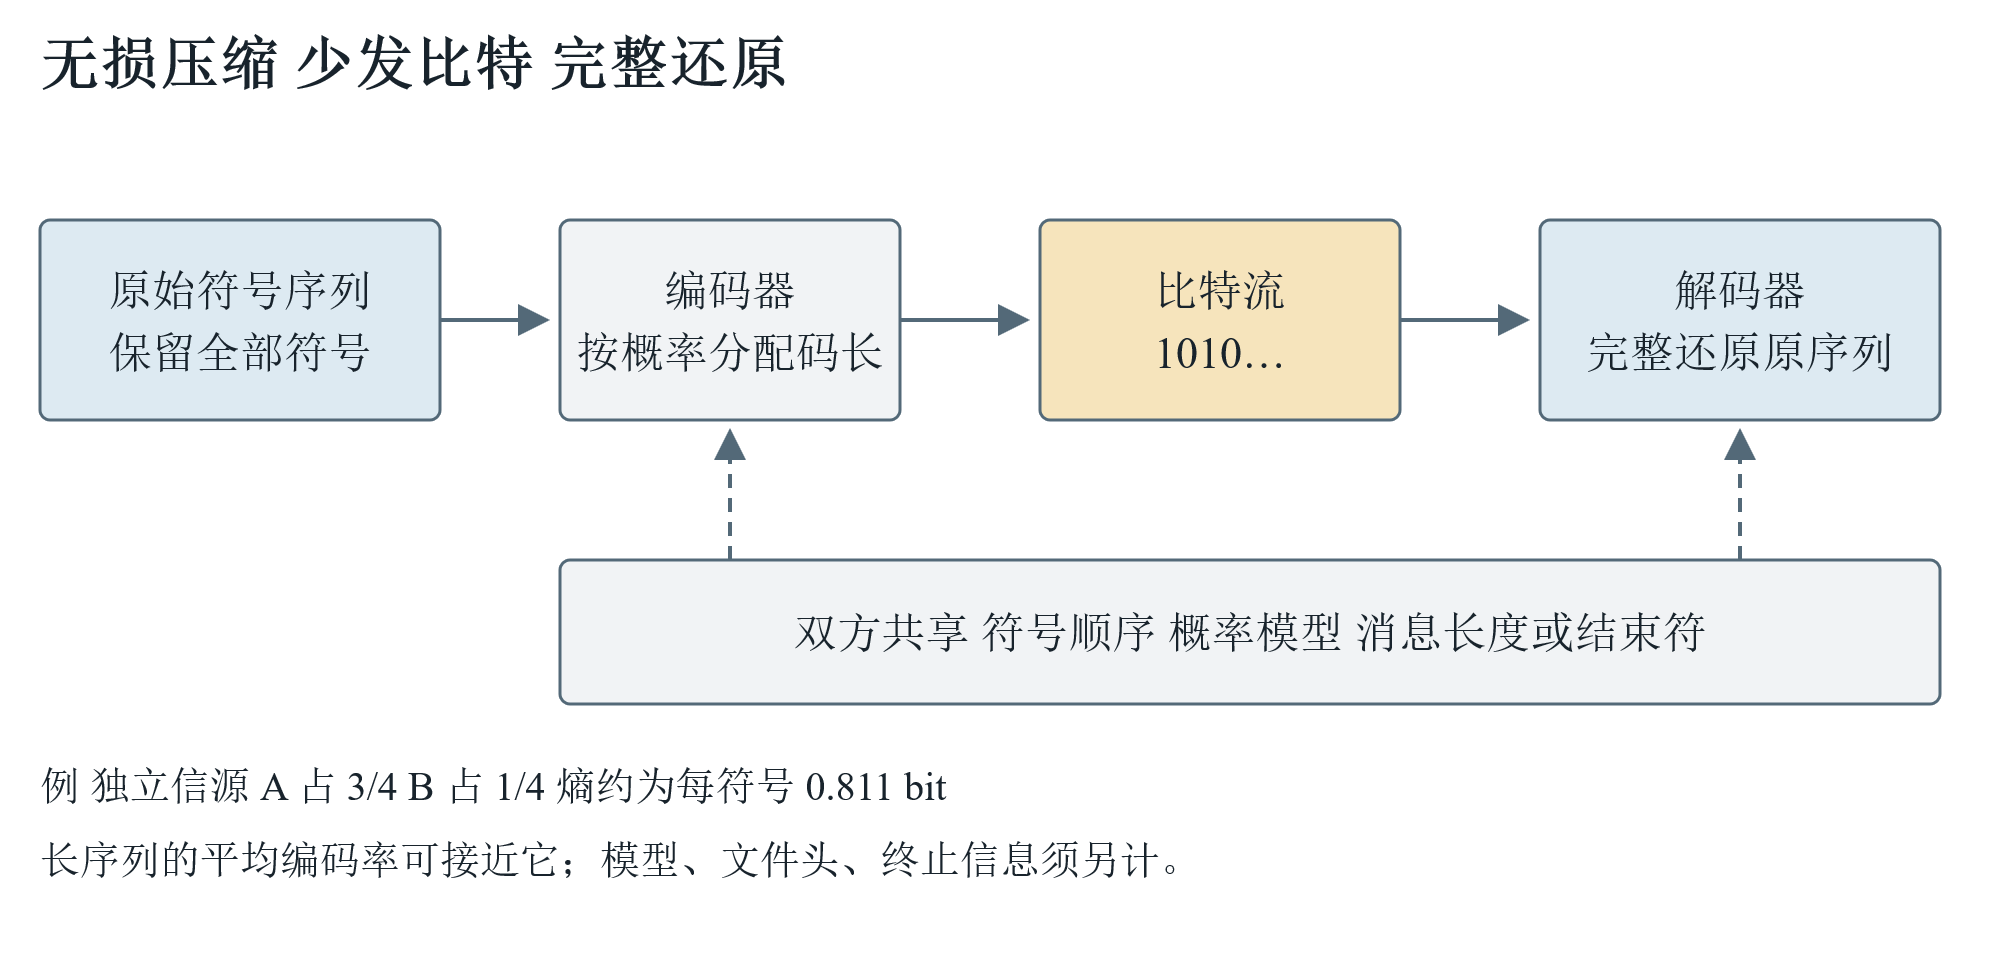
\includegraphics[width=\linewidth]{assets/media/image2.png}
    \caption{无损压缩的目标与两端约定。发送的是足以唯一定位原消息的比特流，接收端必须还原同一条符号序列。}
    \label{fig:无损压缩}
\end{figure}

\textbf{为什么概率能够帮助省位数} 在可唯一解码的约束下，我们不能给每条消息都分配更短的码：短二进制串的数量有限。统计压缩把较短的表示优先留给常见消息，让不常见的消息承担较长的表示，从而降低平均成本。因此，压缩器可能让个别输入变长，尤其是很短或接近随机的输入；无损压缩不承诺每一个文件都缩小。

例如，若符号独立产生且 A 的概率为 3/4、B 为 1/4，我们可以把许多符号一起编码，长消息的平均每符号码率能够接近 0.811 bit，而固定表示是每符号 1 bit。这里比较的是指定信源下的长期平均量；实际有限文件还有终止、对齐和元数据开销。若 A、B 各占一半且彼此独立，就没有这份频率偏斜可利用；如果它们有上下文依赖，仍可以由条件模型进一步利用。

\textbf{算术编码怎样把概率变成比特} 算术编码（arithmetic coding）让编码器与解码器按相同概率划分区间。我们先从 {[}0, 1) 出发，每读一个符号，就按概率切分当前区间，只保留实际符号对应的那一段。待整条消息处理完，编码器发送一段二进制前缀，只要它表示的整个小区间都落在目标区间内，解码器就能确定这条消息。

我们用固定概率走一遍：A 的概率为 0.75，B 为 0.25，消息为 ABA。第一次读 A，保留 {[}0, 0.75)；第二次读 B，保留当前区间最后四分之一，得到 {[}0.5625, 0.75)；第三次读 A，保留当前区间前四分之三，得到 {[}0.5625, 0.703125)。下面每行把上一行选中的区间放大，横轴的尺度随行改变，参考图 \ref{fig:算术编码}。

\begin{figure}[t]
    \centering
    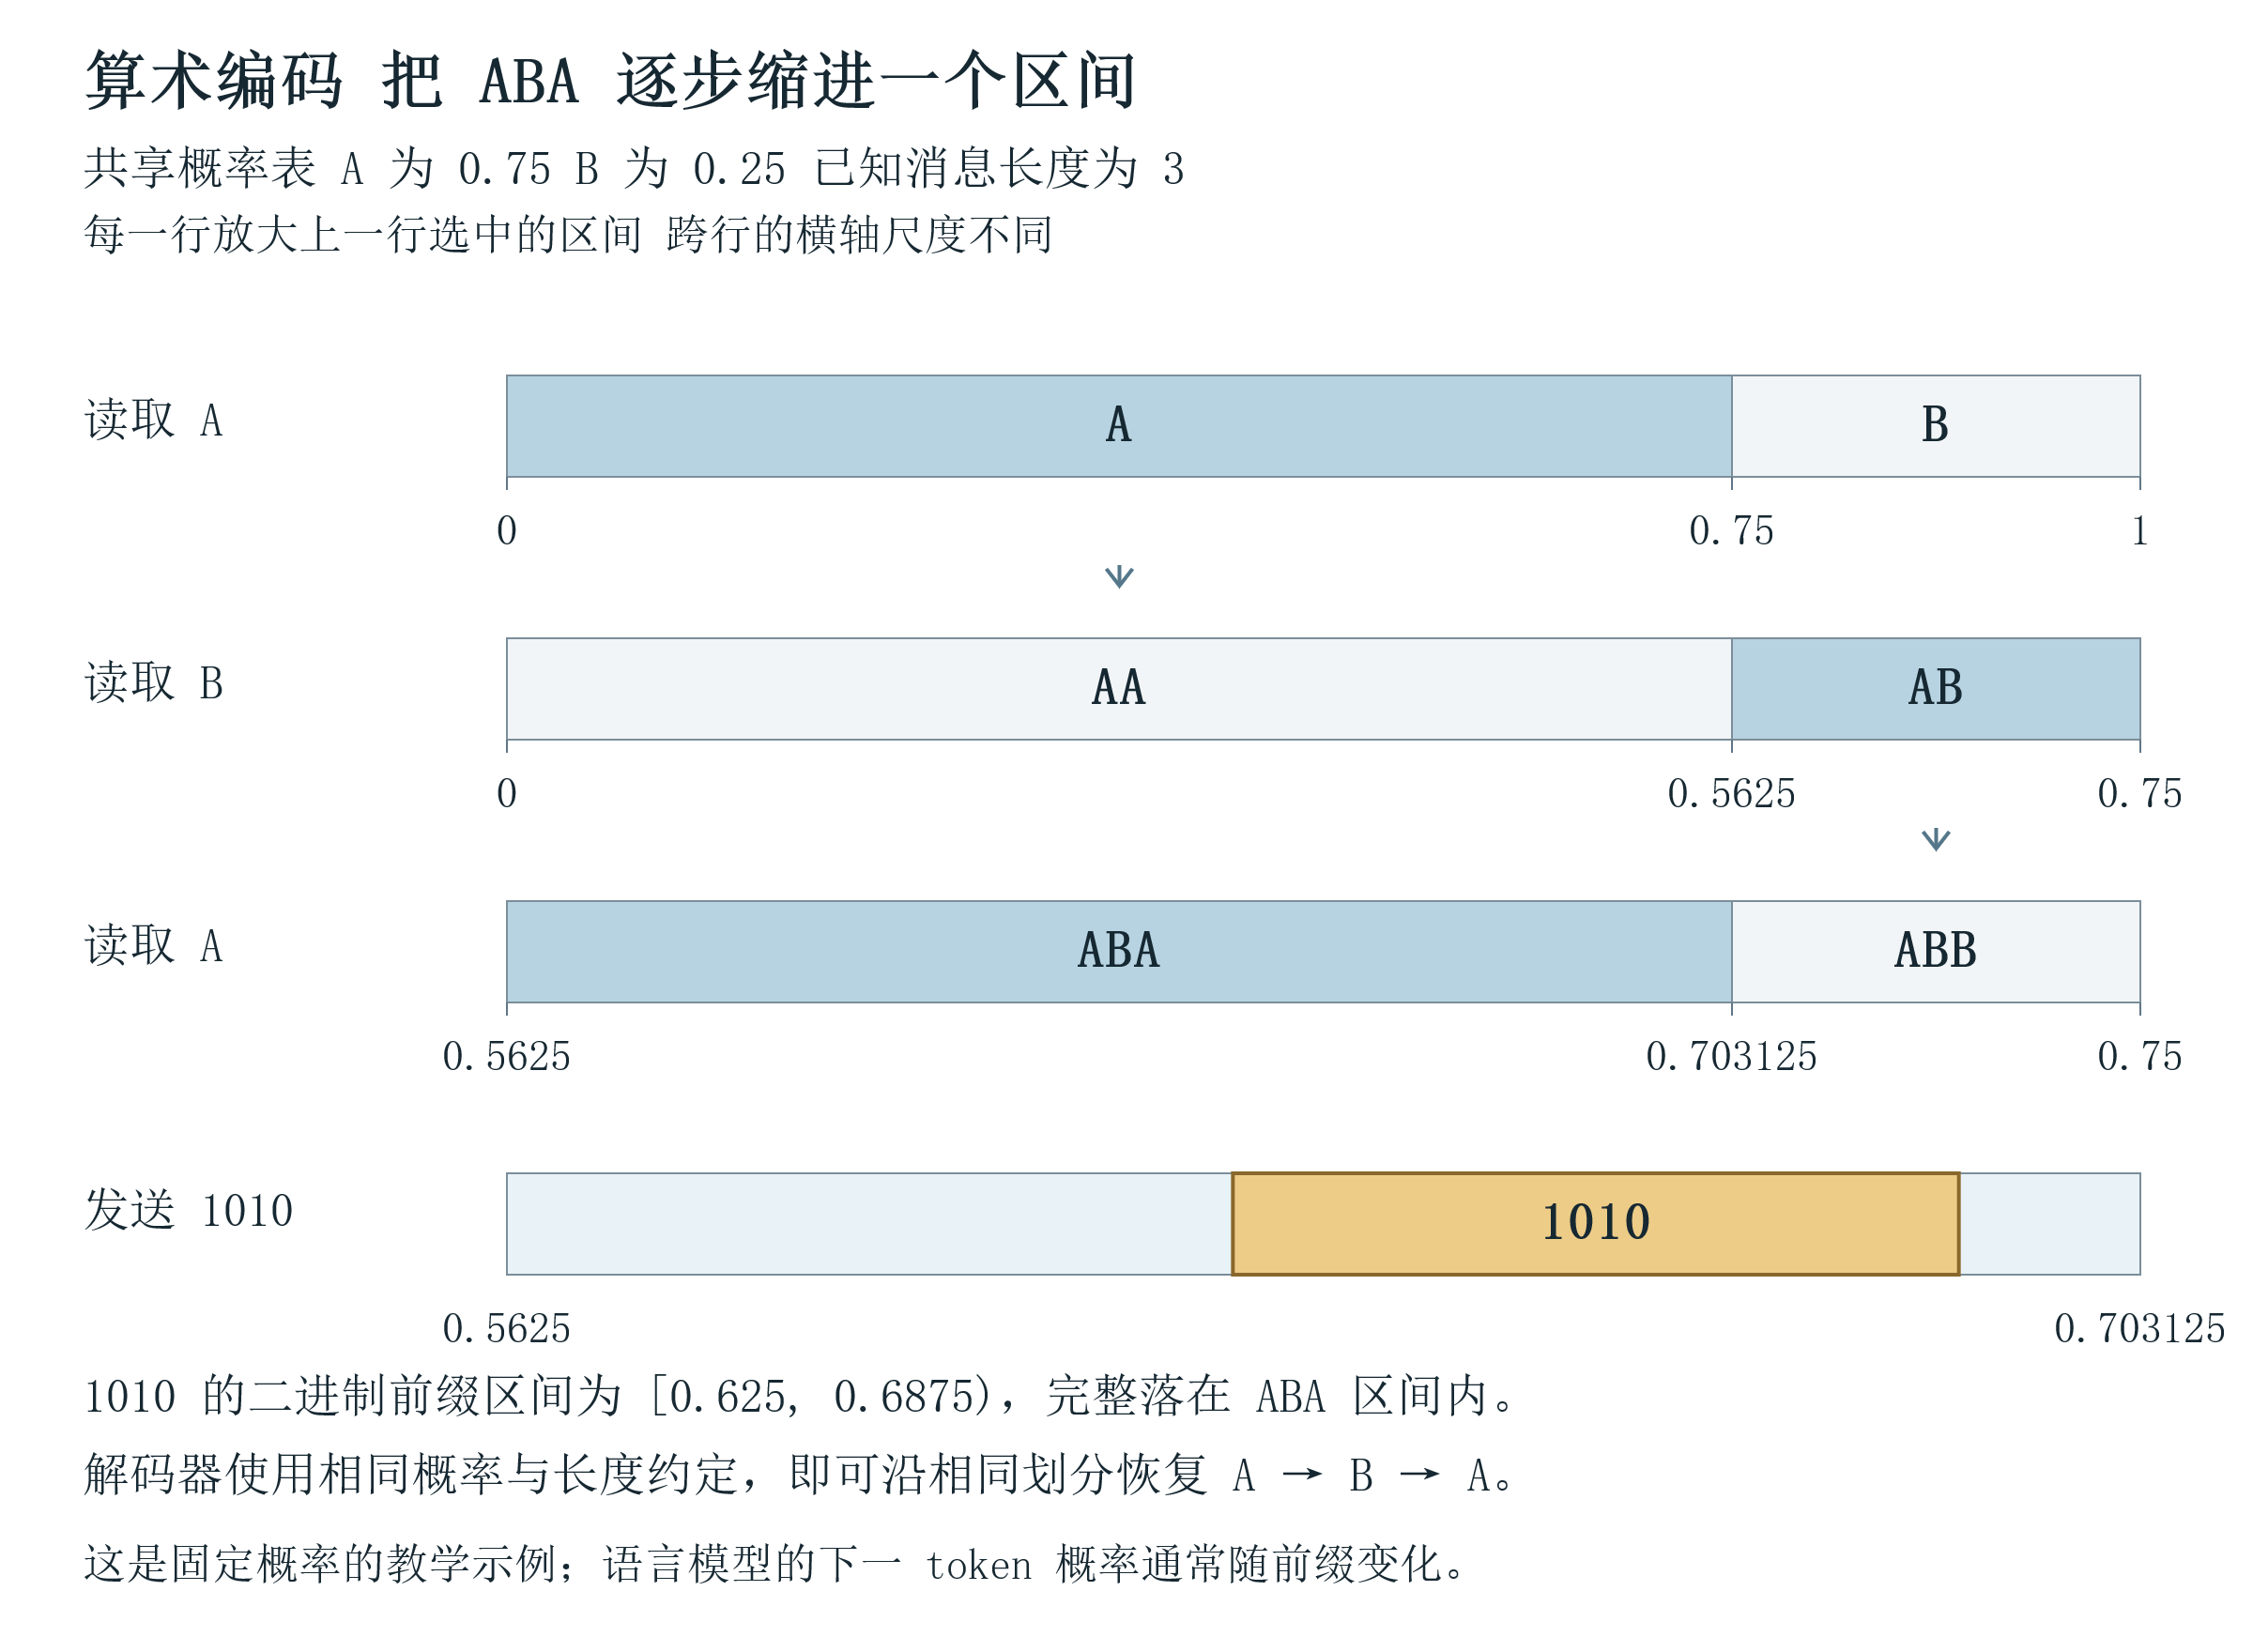
\includegraphics[width=\linewidth]{assets/media/image4.png}
    \caption{算术编码的区间细分。蓝色表示选中的符号区间，橙色表示发送的二进制前缀所对应的区间；跨行不能按图形长度比较绝对宽度。}
    \label{fig:算术编码}
\end{figure}

\textbf{1010 为什么足以还原 ABA} 二进制小数前缀 0.1010 的后续位尚未确定，因此它代表的全部数值位于 {[}0.625, 0.6875)。这个区间完整落在 ABA 的最终区间里。解码器可以取其中一个数，例如 0.625：它位于第一层的 A 区间；继续按同一概率细分，位于第二层的 AB 区间；再细分，位于第三层的 ABA 区间。双方已约定长度为 3，于是停止；若长度未知，就还需要结束符或其他长度协议。实际实现还要处理有限精度和逐步输出比特，我们这里先追踪数学上的区间。

这个例子发送了 4 bit，甚至比二符号固定表示 ABA 所需的 3 bit 更长。这并不矛盾：我们用极短消息展示了可逆机制，尚未展示长期平均压缩收益。若丢掉长度与模型开销、只看漂亮的区间图，就会把``能编码''误当成``这个样本一定更省''。

\textbf{码长怎样回到训练损失} 每选一次符号，区间宽度就乘上该符号的条件概率，所以最终宽度等于整串消息的模型概率。\(m\) 个二进制前缀位对应宽度为 2 的负 \(m\) 次方的区间。为了在目标区间内找到一个可用前缀，所需位数便与概率的以 2 为底负对数相联系。用 \(q\) 表示双方共享的编码模型、\(T\) 表示消息长度，理想信息量写为：
\[l_{q}\left( x_{1:T} \right) = - \log_{2}q\left( x_{1:T} \right) = - \sum_{t = 1}^{T}\log_{2}q\left( x_{t} \mid x_{< t} \right)\]

这里 ℓ 的单位是 bit，x 的下标 1 到 T 表示整串消息，右侧按位置相加；它是理想信息量，不是任意有限文件的最终整数位数。ABA 的概率是 0.75 × 0.25 × 0.75＝9/64，理想信息量约为 2.83 bit，而图中实际选用了 4 位前缀。

现在，前面的交叉熵也有了操作含义。假设真实消息服从 p，而我们按 q 分配码长，那么以 2 为底计算的交叉熵是理想编码长度的平均值；数据自身的熵描述信源不确定性，正向 KL 描述使用不匹配模型额外支付的平均长度。在同一数据上，把真实 token 的预测概率提高，会让对应的理想编码长度降低。

回到语言模型，我们可以让编码器与解码器共享同一个已训练模型。两端从相同起始状态开始；解码出一个 token 后，把它接回前缀，再算出相同的下一步概率。因此，解码器不需要提前知道原文，也不需要靠采样``猜''出原文，而是用收到的编码位从概率区间中确定原 token。两端的分词器、参数、数值实现与结束约定必须兼容。

前面的训练损失使用自然对数，单位为 nat；这里使用以 2 为底的对数，单位为 bit，除以 ln 2 即可把 nat 换成 bit。这个联系说明``预测更准为什么可能让编码更省''，却不表示常规推理会输出压缩文件，也不表示模型权重是训练文本的可逆压缩包，更不能仅据此断言模型已经理解每个事实或解决每道题。知识与推理能力仍要通过独立任务检验。

\section{Transformer 一次前向计算如何完成}\label{Transformer 一次前向计算如何完成}

如果觉得本节讲解过于简单抽象，可以自行查找相关视频学习，重点理解注意力计算、注意力掩码和位置编码ROPE。

知道目标还不够，我们还要知道小助怎样把前缀变成概率。最早的 n 元语法（n-gram）模型只统计有限窗口中的词组合，窗口一长，组合就迅速变稀疏。神经语言模型让上下文共享参数与表示，循环网络再把历史压进状态。变换器（Transformer）架构则让不同位置通过注意力直接交换信息，成为一条适合并行训练的路线。这个历史并非一条必然链，但能帮我们看见每种设计回应的困难。

我们先把 token ID 送入嵌入（embedding）层。它相当于一张可训练查找表：每个 ID 对应一个向量。向量本身没有天然的``第七维就是语法''含义；其意义来自训练后与其他参数的协同。位置编码提供顺序信息，否则模型难以区分``甲帮助乙''和``乙帮助甲''。其中，旋转位置嵌入（Rotary Position Embedding，RoPE）由苏剑林等人在 RoFormer 工作中提出：它按位置旋转查询向量与键向量的表示，让注意力分数能够体现相对位置关系。RoPE 的``相对''性质不等于可以无条件外推到任意长度。

进入一层注意力时，我们把这一层输入的每个位置表示排成矩阵 X。这里的 X 不是原始 token ID，而是已经进入模型计算的向量。同一个 X 分别乘上三套可训练投影矩阵，得到查询（query，Q）、键（key，K）和值（value，V）。它们来自同一批位置，但承担不同计算角色，不能把 Q、K、V 理解成输入中的三种不同词。

我们把三套投影矩阵记为 W 的下标 Q、K、V，投影关系写为：
\[Q = XW_{Q},\quad\quad K = XW_{K},\quad\quad V = XW_{V}\]

若 X 有 n 行，每行具有相同的输入隐藏维度，则查询与键投影把它映射到 d\ensuremath{{}_{k}} 维，值投影映射到 d\ensuremath{{}_{v}} 维；所以 Q、K 都有 n 行、d\ensuremath{{}_{k}} 列，V 有 n 行、d\ensuremath{{}_{v}} 列。这里省略投影偏置，并先讨论一个注意力头。下标用于标识投影角色，不表示它们要对不同的原文分别分词。

把所有位置的 query、key、value 分别排成矩阵 Q、K、V，缩放点积注意力的计算写为：
\[Attention(Q,K,V) = softmax\left( \frac{QK^{\top}}{\sqrt{d_{k}}} + M \right)V\]

上标转置符号表示转置；softmax 对每个 query 的候选 key 分数归一化，再用权重汇总 V。因果掩码 M 在可见位置取 0，在禁止关注的位置用负无穷屏蔽。

其中 d 的下标 k 表示每个 key 的维度；缩放有助于控制点积的数值范围。Q 与 K 的点积是在对应维度相乘后求和，表达一种可训练的匹配分数。M 是掩码。对我们讨论的因果语言模型，未来位置被遮住；训练时即使整段文本同时进入计算，也不能偷看尚未预测的 token。多头注意力让不同子空间并行建立关系。注意力权重是计算的一部分，不能直接当作完整的因果解释。

我们可以把 query 理解为``当前怎样匹配上下文''，key 理解为``每个位置提供怎样的匹配线索''，value 是最终被汇集的信息。这个类比只是计算角色的直觉，向量维度不必对应人类能命名的概念。图 \ref{fig:QKV计算} 把分数、权重和被加权的信息分开。

\begin{figure}[t]
    \centering
    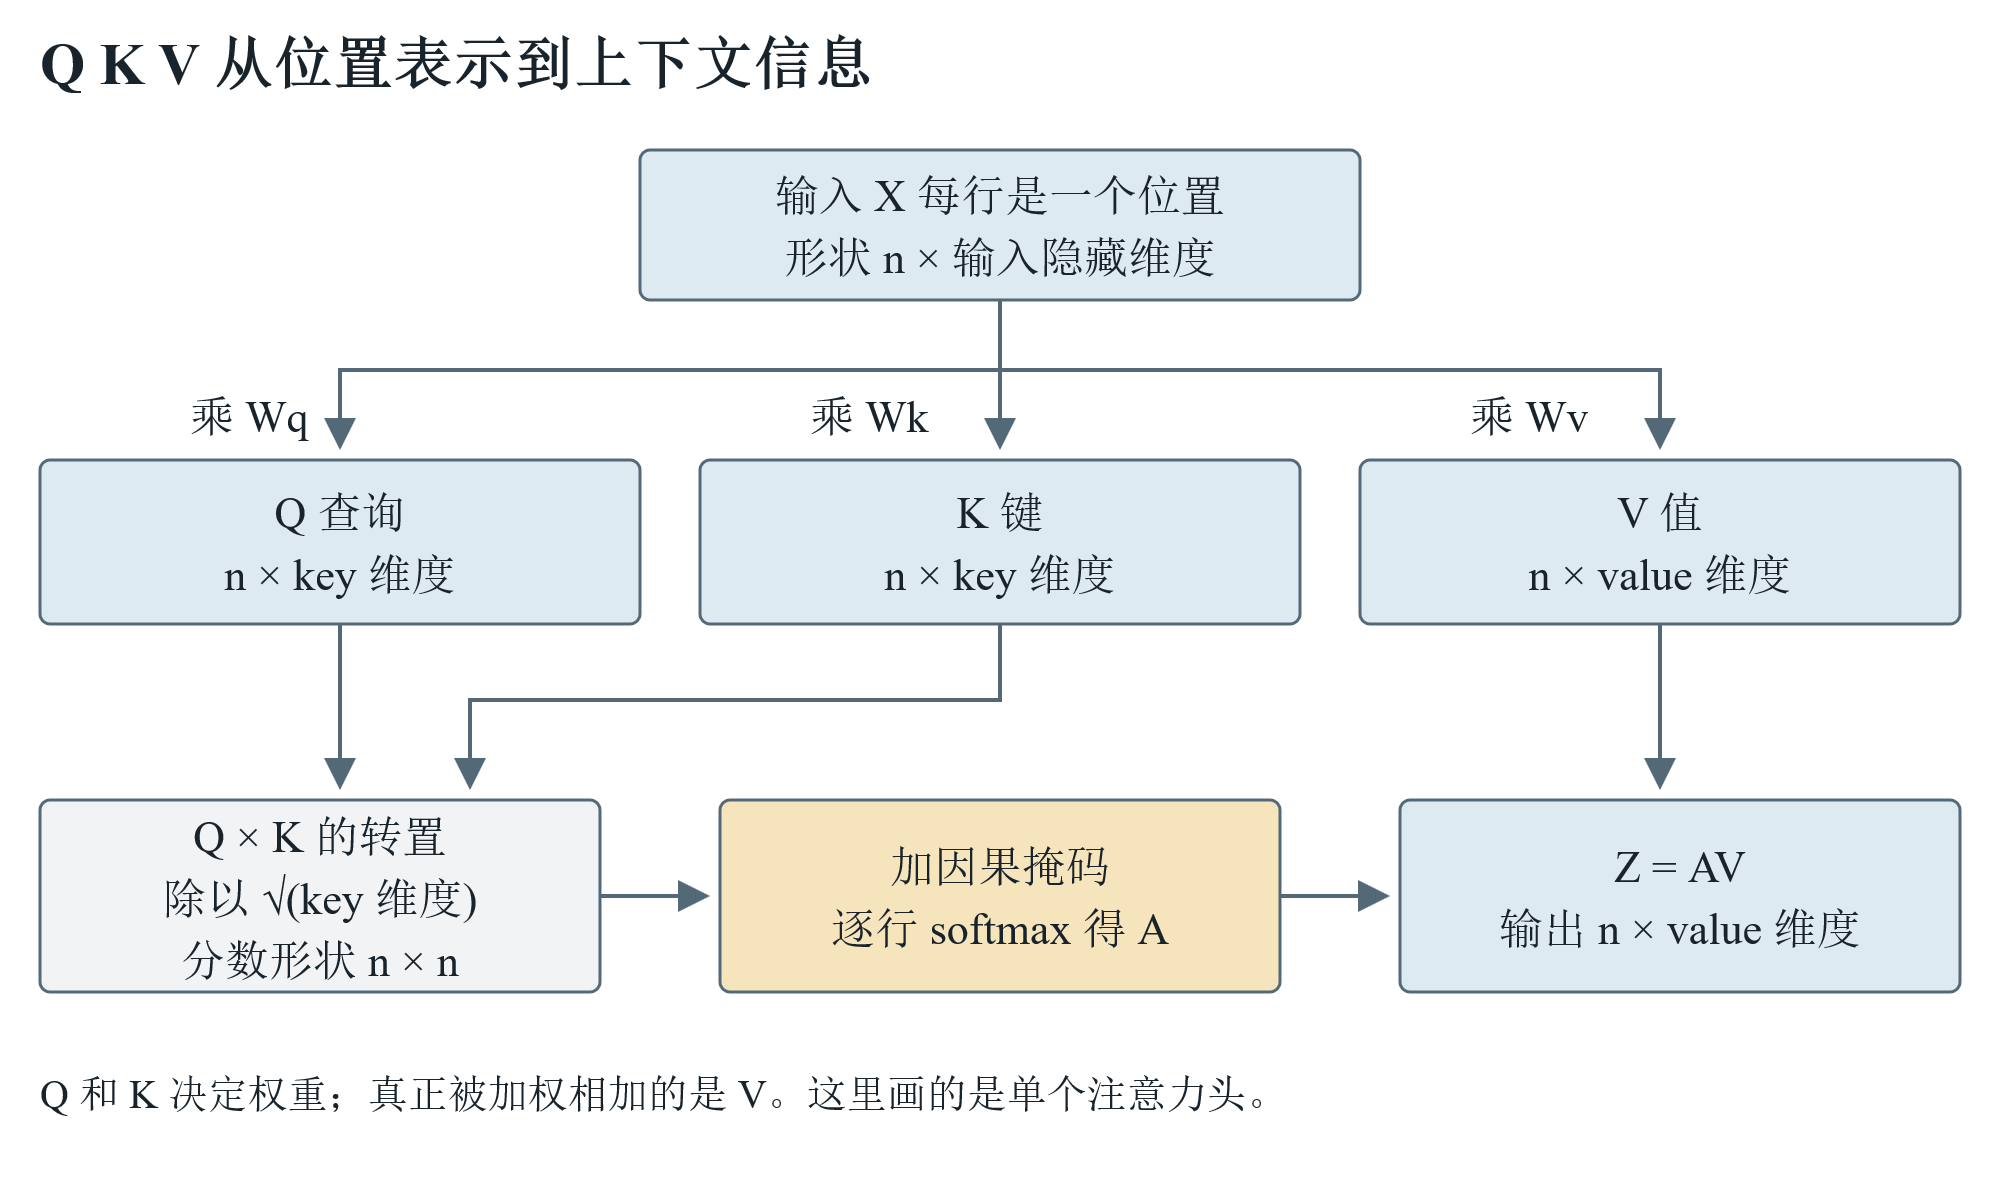
\includegraphics[width=\linewidth]{assets/media/image6.png}
    \caption{单头注意力的数据流。Q 与 K 产生位置之间的分数；掩码与 softmax 得到权重矩阵 A；再由 A 对 V 做加权和。n 是序列长度。}
    \label{fig:QKV计算}
\end{figure}

\textbf{沿着一行真正算一次} 我们暂把``小猫 追球''当作三个玩具 token，站在第二个位置``追''上。本例人为设定了该位置的 q\ensuremath{{}_{2}}，以及三个位置的 key 与 value；这些数只用于复算，并非从真实模型提取。q\ensuremath{{}_{2}} 与三个 key 的点积分别是 1、0、1，除以 √2 后为约 0.707、0、0.707。

第二个位置只能读取第一、第二个位置，第三个位置是未来，因此先把第三个分数置为负无穷，再对这一行做 softmax。前两项得到约 0.670 和 0.330，第三项为 0；最后用这三个权重加权 value，而不是把 key 当作输出。计算结果是约 (1.340, 0.660)。

一个 query 的完整计算：softmax 在允许的位置之间归一化；禁止位置的权重为 0，不能先读未来信息再在输出端补救。

注意，``追''位置更新后的表示可以用于预测后续 token，但当前这次注意力不能把未来``球''的内容拿来使用。训练时整段序列虽然并行送入模型，掩码仍保证每一行只有相应前缀可见。图 \ref{fig:QKV计算} 的 n × n 分数矩阵，就是同时对所有 query 做这样的行计算。

多头注意力把多套投影的结果拼接，再经过输出投影，回到能够与残差相加的隐藏维度。若采用 RoPE，位置相关旋转施加在 Q 与 K 上再计算分数，图 \ref{fig:QKV计算} 省略了这一环节以突出核心数据流；不能因此把位置编码理解成另一份 V。注意力权重也只是这次前向计算的系数，不自动等于因果解释，第九部分会专门检验这一点。

注意力后还有前馈网络、残差连接和归一化。残差让每一层在已有表示上修正，归一化帮助维持适合优化的数值尺度，前馈网络对每个位置做非线性变换。若使用混合专家（Mixture of Experts，MoE）架构，路由器只激活部分专家；这能改变计算与参数容量的配比，但还带来通信、负载均衡和部署问题，并非免费扩大模型。

我们把常见的先归一化（pre-norm）解码器层画在图 \ref{fig:一个Transformer层}。第一条支路通过注意力从其他允许位置取信息，再加回原状态；第二条支路通过前馈网络变换各位置，再加回。图中的归一化位置是这一具体结构的约定，不应推广为所有 Transformer 都完全相同。

\begin{figure}[t]
    \centering
    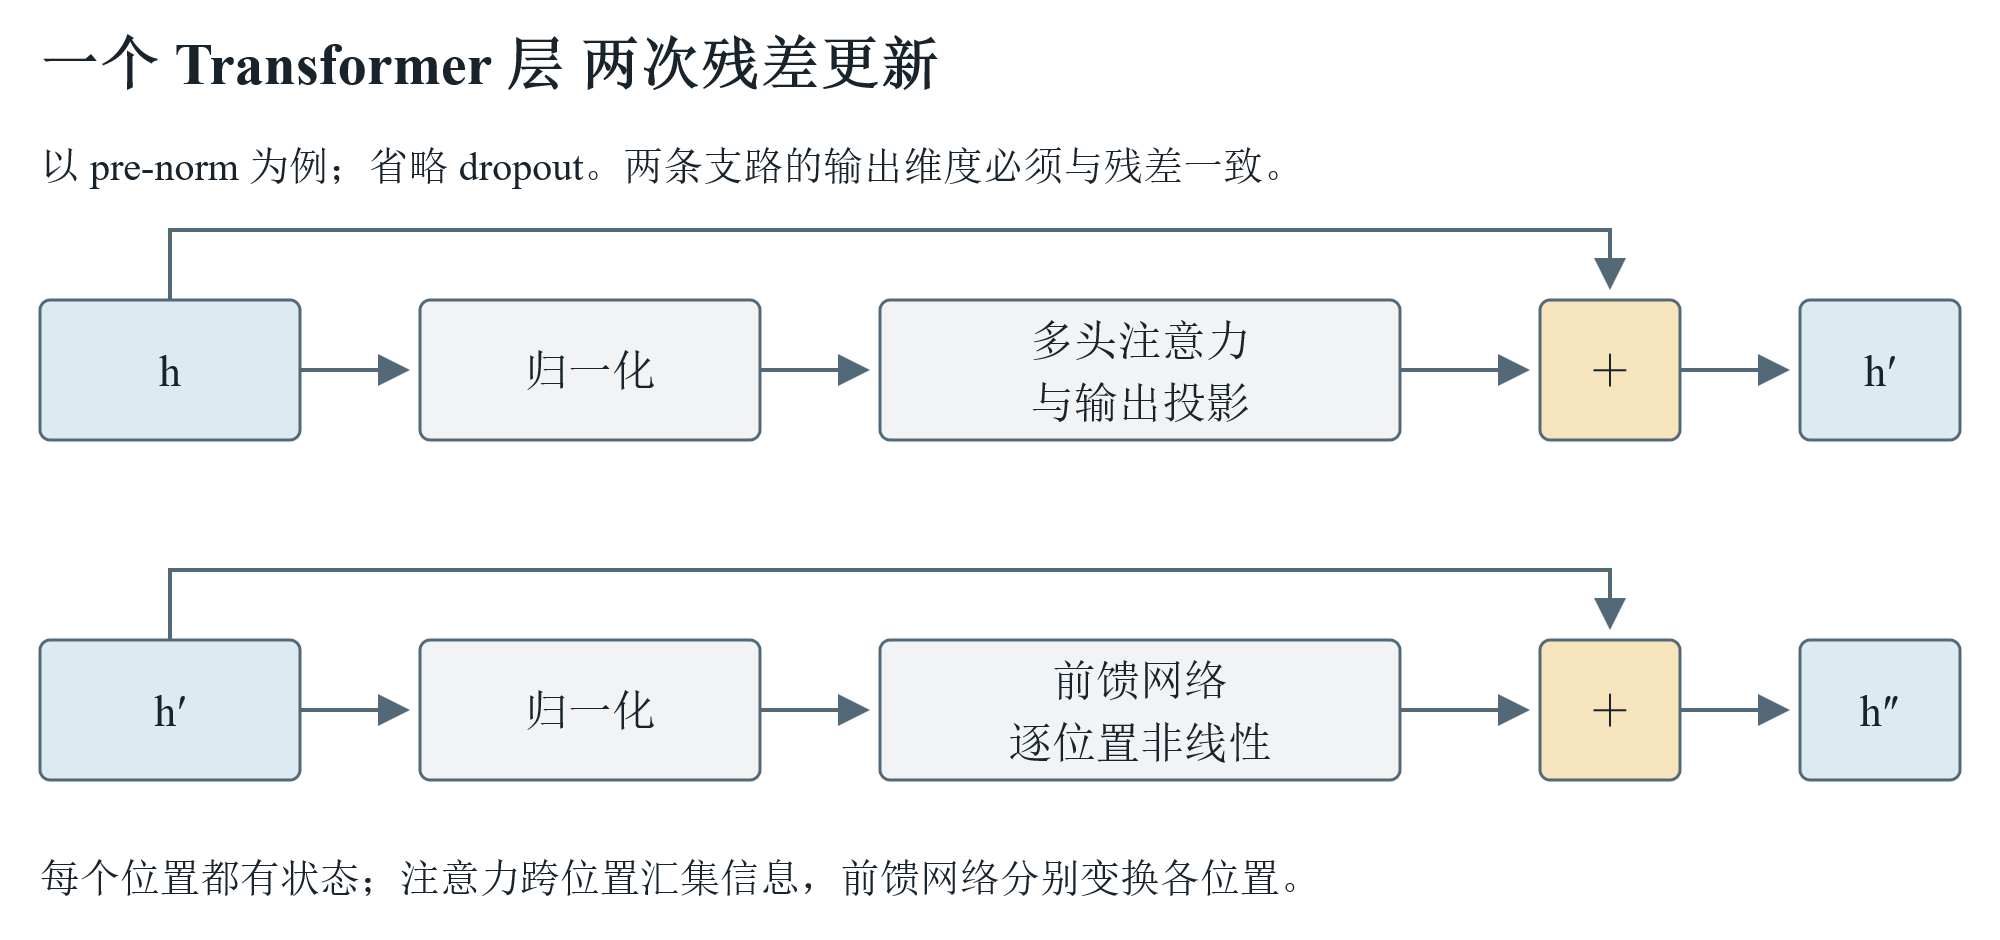
\includegraphics[width=\linewidth]{assets/media/image8.png}
    \caption{一个 pre-norm Transformer 层的两次残差更新。每次加号两侧形状必须一致；多层堆叠后才形成供输出头使用的上下文表示。}
    \label{fig:一个Transformer层}
\end{figure}

经过多层计算，当前位置的隐藏向量被语言模型输出头（Language Model Head，LM head）映射成词表大小的一组未归一化分数（logits）。logits 还不是概率；softmax 才把它们变成总和为 1 的分布。某些模型把输入 embedding 与输出权重绑定，某些不绑定。我们现在能把一轮生成完整地走通：token ID、输入向量、上下文表示、logits、概率，再到下一个 token。

\textbf{配合视频理解} 若 Q、K、V 的矩阵关系仍然抽象，我们可以在 B 站搜索``李宏毅 2021 自注意力机制 Self-attention''，选择包含完整计算过程的课程视频。边看边暂停，画出一次 query 与所有 key 比较、再加权 value 的过程。

\textbf{本节相关资料}
\begin{enumerate}
    \item Vaswani 等，2017，\href{https://arxiv.org/abs/1706.03762}{Attention Is All You Need} 。\textbf{点积注意力里程碑论文，但现在所有的注意力实现都已经不再用这种形式，而是改用 GQA 等高效注意力变体，可自行学习。}阅读重点：注意力计算、多头结构与残差。原论文是编码器解码器结构，阅读时区分它与纯解码器语言模型。
    \item Ba 等，2016，\href{https://arxiv.org/abs/1607.06450}{Layer Normalization} 。阅读重点：归一化解决哪一类优化困难。
    \item 苏剑林等，2021，\href{https://arxiv.org/abs/2104.09864}{RoFormer Enhanced Transformer with Rotary Position Embedding} 。阅读重点：RoPE 怎样通过旋转查询和键，把相对位置关系带进注意力分数。\textbf{中国最重要的大模型研究成果之一，\href{https://spaces.ac.cn/}{苏剑林博客}\footnote{https://spaces.ac.cn/}非常值得阅读。}
\end{enumerate}

\section{预训练与缩放定律 怎样分配训练资源}\label{预训练与缩放定律 怎样分配训练资源}

我们终于可以训练一个toy模型。第一轮输出近乎乱码，训练一段时间后出现词语，再后来句子逐渐连贯。这个过程容易让我们只盯着损失（loss）曲线。可要理解曲线，我们需要先看一次参数更新。

我们从语料抽一个小批次（batch）\footnote{训练时不会一条一条训，而是一次训多条样本，称为一个 batch，与传统机器学习概念一致。}，前向得到预测概率，计算交叉熵，再反向传播得到每个参数对损失的梯度。优化器按学习率调整参数。梯度表示当前位置的局部变化方向，不是对整段知识的显式存储指令。学习率太大可能让训练不稳定，太小可能在有限预算里进展缓慢；有一些缓解方案可以了解：自适应矩估计（Adaptive Moment Estimation，Adam）优化器的解耦权重衰减版本 AdamW（Adam with Decoupled Weight Decay）还会维护优化状态，因此训练显存不只是权重占用。过去很多年工程实践中最常用的是 AdamW，近期出现了一个非常有前景的方法叫 Muon（本节参考论文 3），正在被工业界大规模应用，可以自行了解。

预训练的数据管道同样属于训练方法。我们先清洗编码和模板噪声，去除大量重复，再考虑来源质量、语言比例与许可要求。重复数据会改变训练权重；污染评测集会制造虚假的泛化。把更多低质量文本送进训练，既不等于更多有效知识，也不保证更低的目标任务错误率。

当计算预算有限时，我们有三个可调节预算的选择：模型多大、训练多少 token、使用多少计算。\textbf{缩放定律（scaling laws）}描述在一定实验范围内，损失随这些量变化的经验规律。论文Chinchilla （本节参考文献 1）的重要启发是，\textbf{固定训练计算下，参数和数据需要共同增长}；只扩大模型却训练不足，会浪费潜力，比如对于一个80B模型的训练数据，用来给一个800B的模型训练，模型的最终表现就不会充分发挥。它给出的是在特定设置中拟合出的配比，不是适用于任意数据、架构和部署成本的永久常数。

我们可以把问题变成实验：用同一总计算预算，比较一个大模型少训练与一个小模型多训练。评价时既看验证损失，也看讲题任务。若大模型训练损失更低却验证更差，可能涉及过拟合、数据覆盖或比较预算不公平，不能仅凭参数量推断胜负。

部署会改变最优选择。如果助手要服务许多用户，稍小模型可能值得训练更久，以节省每次推理的成本；如果任务允许调用更强模型，路线又会不同。训练 scaling 与推理时增加采样或思考预算解决的是不同资源分配问题，我们在第七部分再把它们接起来。

\textbf{本节相关资料}
\begin{enumerate}
    \item Hoffmann 等，2022，\href{https://arxiv.org/abs/2203.15556}{Training Compute-Optimal Large Language Models}，也就是 Chinchilla 。阅读重点：固定计算预算如何分配给参数与数据。
    \item Loshchilov 与 Hutter，2017，\href{https://arxiv.org/abs/1711.05101}{Decoupled Weight Decay Regularization}。阅读重点：AdamW 中权重衰减与梯度更新的关系。
    \item Liu 等，2025，\href{https://arxiv.org/abs/2502.16982}{Muon is Scalable for LLM Training}。
\end{enumerate}

\section{幻觉与前缀错位 为什么会连贯地写错}\label{幻觉与前缀错位 为什么会连贯地写错}

预训练后，小助已经能流畅解题。我们问一个编造出来的课程规则：``本课允许迟交几天？''，实际上不允许迟交，但是它也给出一个听上去合理的数字。我们没有把规则交给它，它依然给出答案。这让我们意识到：预测token和确认一个事实对大模型来说是不同的事情。

参数里可以存储和组织大量知识\footnote{大模型训练属于一种信息压缩，把远超参数量的信息压缩到有限的参数中。}，但生成时没有一个自动运行的``事实查表保证''。语料可能过时、相互矛盾或压根不含这个问题的答案。上下文又常暗示``这里应该继续回答''。因此，模型可以生成结构完整但依据不足的内容。我们不能把幻觉说成每个 NTP 模型都必然出现的严格数学定理；更有用的结论是，NTP 本身没有提供逐条事实保证。

另一个风险来自前缀。训练时，我们通常把真实序列的此前 token 交给模型，监督训练下一位置是否出现正确的token。推理时，前缀则包含模型自己刚生成的内容，这就是自回归生成。

小助解题时若第一步误写成``21 除以 3 等于 6''，这一步已经错了，但是后续生成的内容依然看起来合理。训练数据里的标准解从未出现这个前缀，模型不一定学习过从这里纠正错误。训练前缀和实际生成前缀的错位，是暴露偏差（exposure bias）所指的一类问题。

我们把三种幻觉错误分开。1.上下文缺少规则，主要是知识或信息获取问题，即上下文不充分；2.知道题意却输出错误步骤，可能涉及模型学习过的计算与策略；3.第一步错后持续自洽生成，涉及推理错误轨迹的自我恢复与训练分布。对应的实验也不同：1.提供真实资料，观察能否纠正事实；2.提供正确中间步骤，观察能否完成剩余推导；3.故意放入错误前缀，观察能否发现并修正。这里的幻觉问题也是许多公司在面试时经常问的问题。

注意，大模型幻觉之前以及现在都是一个主流的研究方向之一，但随着模型本身智能的增强，幻觉问题很大程度上被缓解，这意味着一些热门问题可能是阶段性的，甚至在一定的历史条件下会被完全消除。

\textbf{本节相关资料}
\begin{enumerate}
    \item Zhang等, 2025, Detecting hallucination in large language models through deep internal representation analysis，\href{https://arxiv.org/abs/2405.19648v1}{https://arxiv.org/abs/2405.19648v1}。我们组张鸾在 2025 年发表的关于幻觉检测的论文。
\end{enumerate}
